% This is "sig-alternate.tex" V1.9 April 2009
% This file should be compiled with V2.4 of "sig-alternate.cls" April 2009
%
% This example file demonstrates the use of the 'sig-alternate.cls'
% V2.4 LaTeX2e document class file. It is for those submitting
% articles to ACM Conference Proceedings WHO DO NOT WISH TO
% STRICTLY ADHERE TO THE SIGS (PUBS-BOARD-ENDORSED) STYLE.
% The 'sig-alternate.cls' file will produce a similar-looking,
% albeit, 'tighter' paper resulting in, invariably, fewer pages.
%
% ----------------------------------------------------------------------------------------------------------------
% This .tex file (and associated .cls V2.4) produces:
%       1) The Permission Statement
%       2) The Conference (location) Info information
%       3) The Copyright Line with ACM data
%       4) NO page numbers
%
% as against the acm_proc_article-sp.cls file which
% DOES NOT produce 1) thru' 3) above.
%
% Using 'sig-alternate.cls' you have control, however, from within
% the source .tex file, over both the CopyrightYear
% (defaulted to 200X) and the ACM Copyright Data
% (defaulted to X-XXXXX-XX-X/XX/XX).
% e.g.
% \CopyrightYear{2007} will cause 2007 to appear in the copyright line.
% \crdata{0-12345-67-8/90/12} will cause 0-12345-67-8/90/12 to appear in the copyright line.
%
% ---------------------------------------------------------------------------------------------------------------
% This .tex source is an example which *does* use
% the .bib file (from which the .bbl file % is produced).
% REMEMBER HOWEVER: After having produced the .bbl file,
% and prior to final submission, you *NEED* to 'insert'
% your .bbl file into your source .tex file so as to provide
% ONE 'self-contained' source file.
%
% ================= IF YOU HAVE QUESTIONS =======================
% Questions regarding the SIGS styles, SIGS policies and
% procedures, Conferences etc. should be sent to
% Adrienne Griscti (griscti@acm.org)
%
% Technical questions _only_ to
% Gerald Murray (murray@hq.acm.org)
% ===============================================================
%
% For tracking purposes - this is V1.9 - April 2009

\documentclass{sig-alternate}
\usepackage{paralist}
\usepackage{color}
\newcommand{\wolfgang}[1]{\textcolor{blue}{\emph{WM: #1}}}
\newcommand{\ariane}[1]{\textcolor{green}{\emph{AK: #1}}}
\newcommand{\daniel}[1]{\textcolor{red}{\emph{DB: #1}}}

\usepackage{url}

\makeatletter
\let\@copyrightspace\relax
\makeatother 

\begin{document}
%
% --- Author Metadata here ---
\conferenceinfo{ANCS}{2011 Brooklyn, New York, USA}
%\CopyrightYear{2007} % Allows default copyright year (20XX) to be over-ridden - IF NEED BE.
%\crdata{0-12345-67-8/90/01}  % Allows default copyright data (0-89791-88-6/97/05) to be over-ridden - IF NEED BE.
% --- End of Author Metadata ---

\title{Efficient Implementation of Dynamic Protocol Stacks}
% in Linux} ?? should we leave it out?

% in Linux\wolfgang{title is ok, but could be more trendy ... I'll think about it}}
%
% You need the command \numberofauthors to handle the 'placement
% and alignment' of the authors beneath the title.
%
% For aesthetic reasons, we recommend 'three authors at a time'
% i.e. three 'name/affiliation blocks' be placed beneath the title.
%
% NOTE: You are NOT restricted in how many 'rows' of
% "name/affiliations" may appear. We just ask that you restrict
% the number of 'columns' to three.
%
% Because of the available 'opening page real-estate'
% we ask you to refrain from putting more than six authors
% (two rows with three columns) beneath the article title.
% More than six makes the first-page appear very cluttered indeed.
%
% Use the \alignauthor commands to handle the names
% and affiliations for an 'aesthetic maximum' of six authors.
% Add names, affiliations, addresses for
% the seventh etc. author(s) as the argument for the
% \additionalauthors command.
% These 'additional authors' will be output/set for you
% without further effort on your part as the last section in
% the body of your article BEFORE References or any Appendices.

\numberofauthors{3} %  in this sample file, there are a *total*
% of EIGHT authors. SIX appear on the 'first-page' (for formatting
% reasons) and the remaining two appear in the \additionalauthors section.
%
\author{
% You can go ahead and credit any number of authors here,
% e.g. one 'row of three' or two rows (consisting of one row of three
% and a second row of one, two or three).
%
% The command \alignauthor (no curly braces needed) should
% precede each author name, affiliation/snail-mail address and
% e-mail address. Additionally, tag each line of
% affiliation/address with \affaddr, and tag the
% e-mail address with \email.
%
% 1st. author
\alignauthor
Ariane Keller\\
       \affaddr{ETH Zurich, Switzerland}\\
       \email{ariane.keller@tik.ee.ethz.ch}
% 2nd. author
\alignauthor
Daniel Borkmann\\
        \affaddr{ETH Zurich, Switzerland}\\
        \affaddr{HTWK Leipzig, Germany}\\
        \email{dborkma@tik.ee.ethz.ch}
% 3rd. author
\alignauthor 
Wolfgang M{\"u}hlbauer\\
       \affaddr{ETH Zurich, Switzerland}\\
       \email{muehlbauer@tik.ee.ethz.ch}
%\and  % use '\and' if you need 'another row' of author names
}
% There's nothing stopping you putting the seventh, eighth, etc.
% author on the opening page (as the 'third row') but we ask,
% for aesthetic reasons that you place these 'additional authors'
% in the \additional authors block, viz.
\date{30 July 2011}
% Just remember to make sure that the TOTAL number of authors
% is the number that will appear on the first page PLUS the
% number that will appear in the \additionalauthors section.

\maketitle
\begin{abstract}

%\wolfgang{I tried to think about an abstract, see next paragraph. Feel free to change ... It's a little bit long, but first sentence can be dropped, etc. Maybe, it's also useful for the intro}
%Beyond doubt, the Internet has grown out of its infancy. Yet, 
Network programming is widely understood as programming strictly defined socket
interfaces. Only some frameworks %(e.g., ANA, Click, Active Networking) 
have made a step
towards \emph{real} network programming by decomposing networking functionality
into small modular blocks that can be assembled in a flexible manner. In this
paper, we tackle the challenge of accommodating 3 partially conflicting
objectives: (i) high flexibility for network programmers,
% and networkapplication designers, 
(ii) re-configuration of the network stack at runtime,
and (iii) high packet forwarding rates.  First experiences with a prototype
implementation in Linux suggest little performance overhead compared to the 
standard Linux protocol stack. 
\end{abstract}

% A category with the (minimum) three required fields
\category{C.2.1}{Computer Communication Networks}{Network Architecture and Design}

\terms{Design, Experimentation, Performance}

\keywords{Network architecture, flexible network stacks, Future Internet experimentation, performance}

\section{Introduction}
Beyond doubt, the Internet has grown out of its infancy and has become a
critical infrastructure for private and business applications. Its success is
largely due to the plethora of transport media 
%(SONET, wired and wireless Ethernet, etc.) 
it uses and to the rich set of network applications 
%(e.g., web, p2p, VoIP, online social networks) 
it offers. Yet, \emph{network programming} is still
mainly about programming sockets that form a strictly defined interface between
the networking (TCP/IP) and the actual application part (Facebook, VoIP, etc.).
What if designers of network applications could even tailor the networking
functionality to their needs? We can just speculate about the resulting
innovations. 

Nowadays, changes in the configuration of a protocol stack usually require
applications or even the operating system to be restarted.  The need for
changing the protocol stack can arise if networking functionality needs to be
patched, if the used encryption method is not considered safe anymore, or when
privacy concerns change. Ideally, applications should not be affected by such
changes.  Therefore, we advocate \textit{run time reconfigurable} protocol
stacks. For example, such protocol stacks can be useful for self-star
properties in computing, since they provide an algorithm that configures and
adapts the protocol stack autonomously.


%Besides allowing application designers to program their own networking stack,
%we envision future Internet applications that \emph{dynamically} adjust their
%network setup/stack during runtime. To give an example: already nowaday's
%websites sometimes redirect users from an HTTP to an SSL-encrypted HTTPS
%connection before sensitive data is exchanged. The step from dynamic
%application-level (SSL-based) to more comprehensive network-layer (IPsec)
%encryption appears small. Yet, enabling a network application to switch to an
%IPSec connection while retaining connectivity is challenging. 

%Additionally, nowadays protocol stacks assume that the timely variances in a
%communication channel can be covered by adaptive parameters inside a single
%protocol. However, this might not be true for long lasting communications (e.g.
%in sensor networks). Network characteristics, privacy or security concerns
%might change with time. The protocol stack should be able to accommodate for
%such changes without the need for restarting the applications. 
%With respect to \emph{real} network programming, related work in this area

Similar objectives were also followed by active networking~\cite{ANSurvey2}, the Click modular router
project\cite{click}, or OpenFlow~\cite{openflow}, etc. 
Yet, we are not aware of any research that has achieved the following three partially conflicting goals:
%The fast speed of the growth of the Internet and the huge effect on everyday life could lead to the thought that it is perfectly designed and nothing should be changed on the underlying architecture. However, researcher are working continuously on new protocols that improve the communication performance for different communication scenarios. Be it in the area of routing, transport or completely new network architectures. The evaluation of such protocols has shown to be difficult as simulations are not realistic enough and as it is difficult to change anything in standard operating systems protocol stacks. To overcome this difficulty some environments dedicated for testing were built, for example Click \cite{click} and openflow \cite{openflow} in the routing area or NetFPGA \cite{netFPGA} for the evaluation of hardware implementations. None of these platforms is specifically designed for evaluating protocols on the end nodes and none of these platforms are designed for an adaptation of the protocol stack at run time. In this paper we present the architecture of a framework that is designed for the following three goals. 
\begin{compactenum}
%\item Provide a platform in which it is easy to test new protocols on end nodes. In order to simplify testing further it should not require any specialized hardware. 
\item Simple integration and testing of new protocols on end nodes on all layers of the protocol stack.
\item Runtime reconfiguration of the protocol stack in order to allow for even bigger flexibility.
\item High performance packet forwarding rates.
%\item Provide a platform that imposes as little overhead as possible. This is required that the evaluation of new protocols delivers meaningful results. 
%\item Provide a platform which allows us to continuously optimize the protocol stack. This is especially useful in mobile scenarios where network characteristics such as delay or packet loss change frequently. Being able to use a protocol optimized for the given network characteristics might improve the connection quality drastically.
\end{compactenum}

In this paper, we propose the \textit{Lightweight Autonomic Network
Architecture (LANA)}. Our architecture borrows ideas from
ANA~\cite{ANAJournal}, where network functionality is divided into
\textit{functional blocks (FB)} that can be combined as required. Each FB
implements a protocol such as \textit{IP, UDP, or content centric
routing.} ANA does not impose any protocols to be used. Rather it provides a framework that allows for the flexible
composition and recomposition of FBs to a protocol stack. This allows for the
experimentation with protocol stacks that are not known by today's standard
operating systems, and it allows for the optimization of protocol stacks at
runtime without communication tear down or application support.  The existing
implementation of ANA shows the feasibility of such a flexible architecture but
suffers sever performance issues. 
%\wolfgang{We need to say what the key
%improvement/change is compared to ANA already here. Not clear yet ->
%kernel-based} 
%In contrast to ANA, the proposed LANA architecture is completely written in the Linux kernel and makes use of its optimized structures for packet handling. Additionally, instead of passing packets by copy between individual blocks we use a strict passing by reference approach.
In contrast to ANA, the proposed LANA architecture relies on a message passing by reference scheme, minimizes the number of threads, and uses optimized packet processing structures provided by the Linux kernel.
Surprisingly, our first experiences with a
prototype implementation suggest that we can offer comparable %functionality and
flexibility as ANA, but at packet forwarding rates comparable to those of the
standard Linux networking stack. 

\section{LANA: Approach}


%\wolfgang{quickly say first why you propose another architecture; e.g., Click configuration if an kernel cannot be changed at runtime or not happy with Ana's performance; it should be come clear that we try to accommodate conflicting objectives, see my abstract}
%LANA provides a framework for setting up protocol stacks not known by todays standard operating systems. Within LANA it is also possible to change the protocol stack at runtime, without communication teardown or application support. These properties build the basis for a networking system that provides protocol stacks that are better targeted to a networking situation than the well known TCP/IP protocol stack.

%LANA provides a framework for setting up protocol stacks not known by 
%todays standard operating systems. Within LANA it is also possible to 
%change the protocol stack at runtime, without communication teardown or 
%application support. These properties build the basis for a networking 
%system that provides protocol stacks that are better targeted to a 
%networking situation than the well known TCP/IP protocol stack.

Generally, the LANA network system is built similarly to the network subsystem of the Linux kernel.
Applications can send and transmit packets via the BSD socket interface. The actual packet processing is done in a \textit{packet processing engine (PPE)} in the kernel space. An overview of the architecture is presented in Figure \ref{fig:architecture}.

%\daniel{too much is said about the vlink interface. I'd rather save the words for the PPE or functional blocks. I think about a better paragraph for tomorrow}

The hardware and device driver interfaces are hidden from the PPE behind a \textit{virtual link interface}, which allows for a simple integration of different underlaying networking technologies such as Ethernet, Bluetooth or InfiniBand.
% Additionally, virtual link interface devices are represented as usual kernel networking devices and can be managed with standard tools such as \texttt{ifconfig} or \texttt{ethtool}.

Each functional block is implemented as a Linux kernel module. 
Upon module insertion a constructor for the creation of an instance of the FB is registered with the LANA core. Upon configuration of the protocol stack the instances of the FBs are created. The instances register a \textit{receive function} with the PPE. This function is called when a packet needs to be processed.
%It offers a \textit{receive handler} that is invoked by the PPE upon packet processing. Functional blocks are built as objects of a specific type. Their build handlers are registered to the LANA core during module registration. 

Functional blocks can either drop a packet, forward a packet to either ingress or egress direction, or duplicate a packet. After having processed a packet, the FB returns the identifier of the next FB that should process this packet. In addition, FBs belonging to the virtual link interface will queue the packets in the network drivers transmit queue and FBs communicating with BSD sockets will queue the packets in the sockets receive queue.

The PPE is responsible for calling one FB after the other and for queuing packets that need to be processed.

%Data is transmitted between the functional blocks by function calls and is 
%therefore not being copied between functional blocks.
% A network packet is 
%processed by the LANAs packet processing engine, which calls receive handlers 
%of functional blocks that are bound to each other in the processing path. Data is then 
%either forwarded to the subsequent functional block or discarded. A certain
%path can be traversed in ingress or egress direction, thus functional
%blocks can also flip the packets direction within the packet processing engine.
%Moreover, the packet processing engine has per-CPU backlog queues so that
%functional blocks which spawn new network packets can enqueue the like for
%processing.

%There are two special functional blocks - those of the virtual link interfaces 
%communicating with a network driver and those communicating with BSD sockets.
%These functional blocks push network packets either in the drivers transmit 
%queue or in the sockets receive queue.

\begin{figure}
\centering
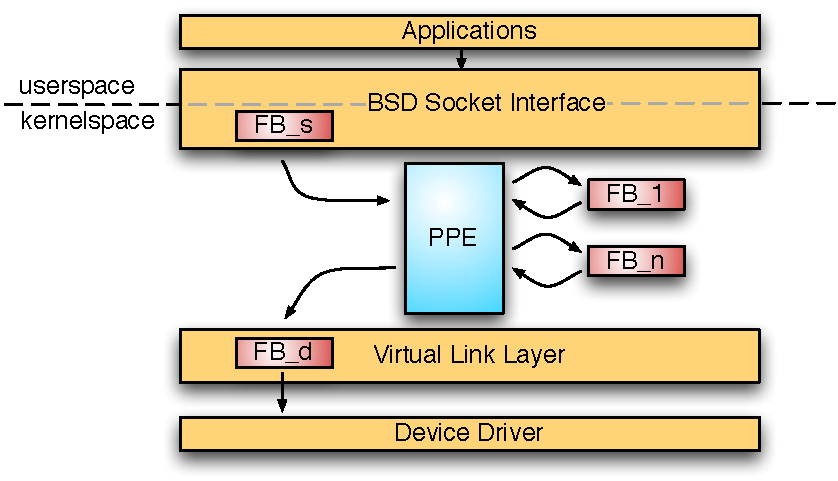
\includegraphics[width=0.31\textwidth]{figures/data_flow.pdf}
\vspace{-0.1cm}
\caption{Packet flow in LANA}
\label{fig:architecture}
\vspace{-0.2cm}
\end{figure}
%\begin{figure}
%\centering
%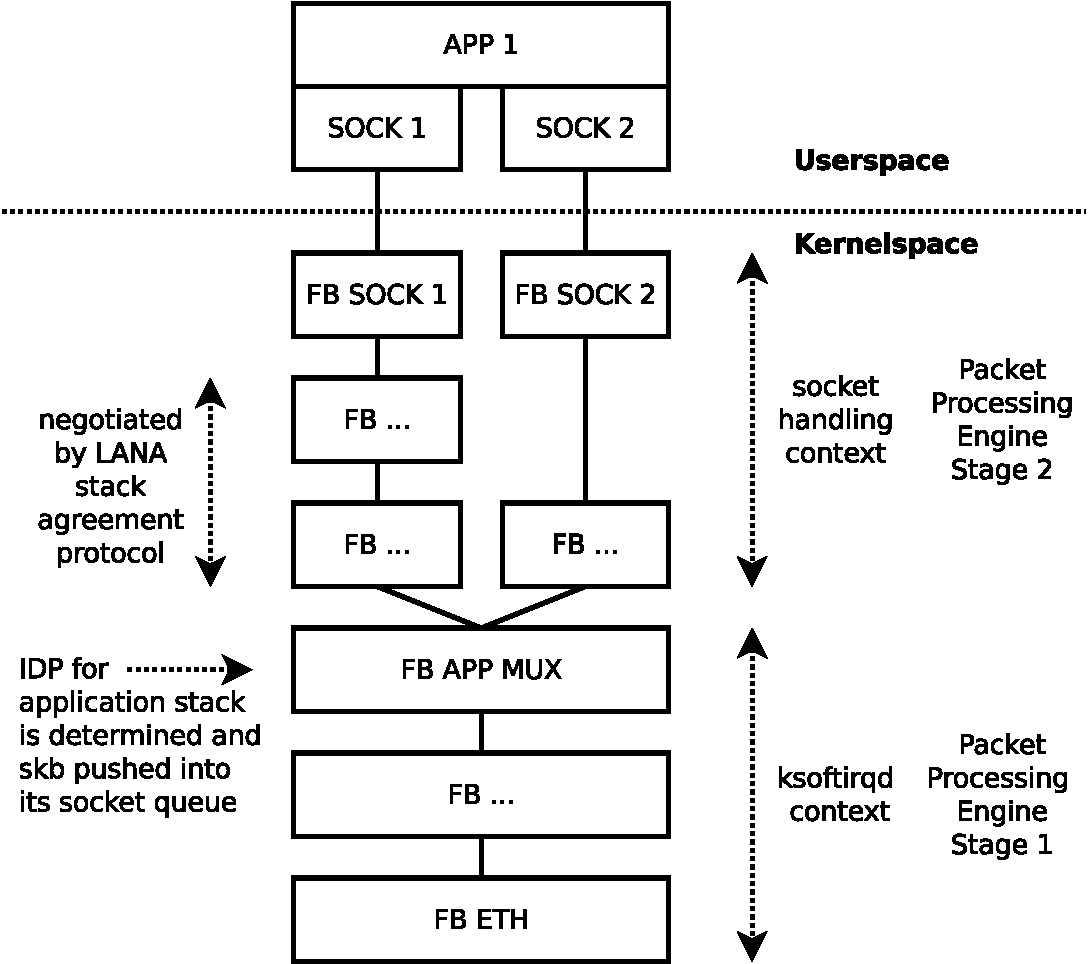
\includegraphics[width=0.4\textwidth]{figures/stack.pdf}
%\caption{Lana protocol stack showing in which contex which functionality is implemented}
%\label{fig:stack}
%\end{figure}

\subsection{Implementation}
%\subsubsection*{Configuration Interface}
The protocol stack can be configured from user space with the help of a 
command line tool. The most important commands are summarized below.
\begin{compactitem}
\item \texttt{add}, \texttt{rm}: Adds (removes) an FB from the 
      list of available FBs in the kernel. 
\item \texttt{set}: sets properties of an FB with a 
      \texttt{key=value} semantic.
\item \texttt{bind}, \texttt{unbind}: Binds (unbinds) an FB 
      to another FB in order to be able to send messages to it. 
\item \texttt{replace}: Replaces one FB with another 
      FB. The connections between the blocks are maintained. 
      Private data can either be transferred to the new block or dropped.
%\item \texttt{subscribe}, \texttt{unsubscribe}: Subscribes (Unsubscribes) one 
%      functional block to receive event messages from another functional block.
%      (An implicit subscribtion (unsubscribtion) is done on bind (unbind).)
\end{compactitem}
Within the Linux kernel the notification chain framework is used to propagate those configuration messages to the individual FBs. 
%This framework is also used to distribute other, internal, configuration messages. 

%\subsubsection*{Available Software}
The current software is available under the GNU General Public License from 
\cite{lana}. In addition to the framework, it also includes five functional 
blocks: Ethernet, Berkeley Packet Filter, Tee (duplication of packets), Packet 
Counter and Forward (an empty block that forwards the packets to 
another block). The framework does not need any patching of the Linux kernel
but it requires a new Linux 3.X kernel.

\subsection{Improving the Performance}
We have evaluated different options for the integration of the PPE with
the Linux kernel. We summarize our insights to provide guidance for researchers
who apply fundamental changes on the Linux protocol stack.

We compared the maximum packet reception rate of the Linux kernel while not
doing any packet processing with LANA. In LANA packets are forwarded between
three FBs that do only packet forwarding. 

%Our goal was to be able to process as many \textit{minimum sized Ethernet frames} 
%as the Linux kernel is able to process. In order to compare the performance of 
%the Linux Kernel and the performance of our engine we have bypassed all packets 
%from the Linux Kernel protocol stack into the LANA stack via a
%\texttt{netdev\_rx\_handler} in bottom half context as soon as they arrived.

%In our system the packets were processed by the \texttt{fb\_eth} functional 
%block followed by two \texttt{fb\_dummy} functional blocks that were simply 
%forwarding the packets. We can distinguish the following three approaches:
\begin{compactitem}
\item One high priority LANA thread per CPU achieves approx. half the performance of the default Linux stack. The performance degradation is due to 'starvation' of the software interrupt handler (ksoftirqd). Changing the priority of the LANA thread only slightly increases the throughput.
% (since the ksoftirqd is a low-priority thread).
\item Explicit preemption and scheduling control achieves approx. two third of the performance of the default stack. The performance degradation is due to scheduling overhead. 
\item Execution of the PPE in ksoftirqd context achieves approx. $95\%$ of the performance of the default stack.
\end{compactitem}

The corresponding numbers are listed in Table \ref{tab:performance}.
\begin{table}[t!]
\begin{tabular}{ l r }
Mechanism & Performance\\
\hline
Kernel threads (high priority) & 700.000\\
Kernel threads (normal priority) & 750.000\\
Kernel threads (controlled scheduling) & 900.000\\
Execution in ksoftirqd & 1.300.000\\
Linux kernel networking stack & 1.380.000\\
\end{tabular}
\vspace{-0.1cm}
\caption{Performance evaluation in pps with 64 Byte packets.
% The evaluation was done with the kernel packet generator \texttt{pktgen} on two directly 
%connected machines with 
(Intel Core 2 Quad Q6600 with 2.40GHz, 4GB RAM, Intel 82566DC-2 NIC, Linux 3.0rc1)}
\label{tab:performance}
%\vspace{-0.5cm}
\end{table}
%\vspace{-0.1cm}
\section{Conclusions and Future Work}
We described how to implement a flexible protocol stack with similar
performance as the default Linux stack. Its flexibility allows to
include and test protocols, yet to be developed, and to change the protocol
stack at runtime. In contrast to TCP/IP, our proposed solution allows to tailor
the networking layer for the needs of a particular networking situation. In the
short-term, we will compare LANA performance achieved in real scenarios with
other systems (e.g., default Linux stack, Click router, etc.).  In the
mid-term, we plan to work on mechanisms that automatically configure protocol
stacks based on the needs of applications and networks. In the long-term, we
envisage a system that requires less configuration as compared to today's
networks and that is able to adapt itself to changing network conditions.   



%In the midterm we will develop a mechanism that automatically sets up a protocol stack for an Application whereby the Application can specify some characteristics the communication channel should have, but not exactly how this has to be achieved. For example the application could require a "reliable communication channel" and a controller would choose between different protocols that provide reliability (e.g., one for wired communication, one for wireless communication, one for wireless, multi-hop communication). The setup of the protocol stack will have to be negotiated between the source and destination node. 

%\end{document}  % This is where a 'short' article might terminate

%ACKNOWLEDGMENTS are optional
\section{Acknowledgments}
This research has received funding from the European Union 7th Framework Programme (grant $n^o 257906$).
%
% The following two commands are all you need in the
% initial runs of your .tex file to
% produce the bibliography for the citations in your paper.
\bibliographystyle{abbrv}
\bibliography{epics}  % sigproc.bib is the name of the Bibliography in this case
% You must have a proper ".bib" file
%  and remember to run:
% latex bibtex latex latex
% to resolve all references
%
% ACM needs 'a single self-contained file'!
%
%APPENDICES are optional
%\balancecolumns
\end{document}
